%   This is a template for a senoir honours project report.
\documentclass[a4paper,12pt]{article}
\usepackage{fullpage}
\usepackage[pdftex]{graphicx}
\usepackage{float}
\usepackage{amsmath, amsthm, amsfonts, amssymb}
\usepackage{multicol}
\usepackage{xcolor}
\usepackage{subfiles}
\usepackage{caption}
\usepackage[a4paper, total={6in, 9in}]{geometry}
\usepackage[version=4]{mhchem}
\usepackage[hyphens]{url}
\usepackage{hyperref}
\usepackage{eurosym}
\usepackage{soul}
\usepackage{siunitx}
\usepackage{booktabs}
\usepackage[numbers]{natbib}
%Added to space out paragraphs
\usepackage{parskip}
\usepackage{subcaption}
\usepackage{amssymb}



\def\reac{$^{21}$Ne(p,$\gamma)^{22}$Na reaction }
\def\Q{Q_{\rm{value}}}

%
%                       This section generates a title page
%                       Edit only the sections indicated to put
%                       in the project title, your name, supervisor,
%                       project length in weeks and submission date
%
\begin{document}
\pagestyle{empty}                       % No numbers on title page      

\par\noindent\includegraphics[width=14cm]{}

\par\noindent                                           % Centre Title, and name
\vspace*{1cm}
\begin{center}
        \bf Senior Honours Project\\
        \Large\bf Stellar Nucleosynthesis of $^{22}$Na: Calculating Resonance Strength at Astrophysical Energies          % Replace with your title
\end{center}
\vspace*{0.5cm}
\begin{center}
        \bf Abhinav Datla\\                               % Repace with your name and
        March 2024                                   % Submission Date
\end{center}
\vspace*{5mm}
%
%                       Insert your abstract HERE                
\begin{abstract}
This report analyses the \( ^{21}\text{Ne}(p,\gamma)^{22}\text{Na}\) reaction, pivotal for understanding stellar nucleosynthesis within the Neon-Sodium cycle. Using data from the Laboratory for Underground Nuclear Astrophysics (LUNA), we calculate the reaction's resonance strength at a resonance energy of 271 keV. Analysis at this resonance involved an evaluation of different steps of the experiment and subsequent data analysis, with the result being a foundation for obtaining a total reaction rate for the \reac, as well as a deeper understanding of the steps taken to quantify thermonuclear reactions.
\end{abstract}

\vspace*{1cm}

\subsubsection*{Declaration:}

\begin{quotation}
  I declare that this project and report is my own work.
\end{quotation}

\vspace*{2cm}
{\bf{Signature:}}\textit{Abhinav Datla}\hspace*{8cm}\textbf{Date}:  31/3/2024         % You can include a scanned version 
                                                 % of you siganture here, or comment 
                                                 % this line out

\vfill
{\bf Supervisors:}                % Change to suit

\textbf{10 Weeks}                                         % Change to suit
\newpage
%
%                       End of Title Page
\pagestyle{plain}                               % Page numbers at bottom
\setcounter{page}{1}                            % Set page number to 1
\tableofcontents{}  
\newpage


\section{Introduction}

Nucleosynthesis is the cosmic process responsible for forming chemical elements from nuclear reactions.  The first acts of nucleosynthesis were made by the Big Bang which formed the lightest elements -hydrogren, helium, lithium, but the origin of the heavier elements was shrouded in mystery.  This was until 1957, when a paper by Burbidge, Burbidge, Fowler, and Hoyle (B$^{2}$FH), proposed that these heavier elements were actively being synthesized in the interiors of evolving stars.  This greatly shifted scientific perspective, setting stars as one of the primary origins of matter \citealp{RolfsRodney1988}.  

The nucleosynthesis of elements in stars hinges on the thermonuclear reactions that occur.  Different reactions are initiated at different stages of the star's life cycle, which changes based on the core temperature.  Selecting a particular reaction to analyze is based on a number of factors, some of which may be the feasibility of replicating it in a controlled environment, or the applications of the resultant isotope itself.  Most importantly however, is its cosmic \textit{footprint}, i.e. certain distinctive properties of the reaction that allow it to be observed with low uncertainty.  For this reason, the $^{21}$Ne(p,$\gamma)^{22}$Na reaction is of significant interest, explained in detail in section \ref{Background}.  As far as what "analyzing" a reaction entails, critical stellar features such as lifetime, nucleosynthesis, and producing nuclear energy is based on the magnitude of the reaction rate per particle pair, $<\sigma\upsilon>$ \citealp{RolfsRodney1988}.

The Laboratory for Underground Nuclear Astrophysics (LUNA) allows scientists to replicate the conditions present inside stars with exceptional accuracy.  The reproduction of these reactions allows us to refine the measurement of the reaction rate.  The goal of this report will be to analyze experimental data of the $^{21}$Ne(p,$\gamma)^{22}$Na reaction from LUNA, and calculate the resonance strength $\omega\gamma$, which leads to the reaction rate  $<\sigma\upsilon>$. We will begin with a description of the $^{21}$Ne(p,$\gamma)^{22}$Na reaction's astrophysical context as well as calculating the thermonuclear reaction rate in section \ref{Background}. Then, section \ref{luna} will discuss the experimental setup in detail and the last section, \ref{data} will provide the details of the data analysis as well as the results that were obtained.  


\section{Background and Astrophysical Motivation}\label{Background}

\subsection{Thermonuclear Reaction Rate}\label{therm}



For a single thermonuclear reaction, the energy released ($Q_{\rm{value}}$), distinguishes the two main types of reactions: positive $Q_{\rm{value}}$ $\rightarrow$ exothermic, negative $Q_{\rm{value}}$ $\rightarrow$ endothermic.  The \reac is exothermic and its $\Q$ is calculated using the starting masses of the elements as follows,

\begin{equation}
    \Q = [(m_{\rm{^{21}Ne}} + m_{\rm{p}}) - (m_{\rm{^{22}Na}}+m_{\rm{\gamma}})]c^2
\end{equation}

where the $\Q$ is obtained in units of MeV, $m_x$ represents the mass of their respective elements in amu(and $m_{\gamma}$ is massless), and $c^2$ $\approx$ 931.5 $\frac{MeV}{u}$. The $\Q$ will be relevant in proceeding sections as we discuss the resonances of the \reac.  We will turn our focus to the reaction rate.    

For a single resonance, the reaction rate \(\langle \sigma v \rangle\) can be derived by considering the Maxwell-Boltzmann distribution for particle velocities and the resonant nature of the cross-section \(\sigma(E)\):
\begin{equation}
\langle \sigma v \rangle = \left( \frac{8}{\pi \mu} \right)^{1/2} \left( \frac{1}{kT} \right)^{3/2} \int_0^\infty \sigma(E) E \exp \left( -\frac{E}{kT} \right) dE.
\end{equation}
Here, \(\sigma(E)\) is represented by the Breit-Wigner formula near the resonance energy, \(E\) is the center-of-mass energy of the interacting particles, \(k\) is the Boltzmann constant, \(T\) is the temperature, and \(\mu\) is the reduced mass of the system. This integral evaluates the reaction rate over all energies, accounting for the probability of particle interaction at a given energy, as dictated by the Maxwell-Boltzmann distribution.  The full derivation of the equation is found in \citealp{RolfsRodney1988}.

For a reaction with multiple resonances, we consider each resonance's contribution to the cross-section \(\sigma(E)\). The cross-section near a resonance can be described by the Breit-Wigner formula, which for the \(i\)-th resonance is:
\begin{equation}
\sigma_i(E) = \frac{\pi \hbar^2}{2 \mu E} \frac{\omega \gamma_i}{(E - E_i)^2 + (\Gamma_{i,\text{total}}/2)^2},
\end{equation}
where \(\omega \gamma_i\) is the resonance strength, \(E_i\) is the resonance energy, and \(\Gamma_{i,\text{total}}\) is the total width of the resonance. The reaction rate for multiple resonances becomes a sum over all individual resonance contributions:
\begin{equation}
\langle \sigma v \rangle = \left( \frac{8}{\pi \mu} \right)^{1/2} \left( \frac{1}{kT} \right)^{3/2} \sum_i \int_0^\infty \sigma_i(E) E \exp \left( -\frac{E}{kT} \right) dE.
\end{equation}
Substituting the Breit-Wigner formula for \(\sigma_i(E)\) into the integral, we get:
\begin{equation}
\langle \sigma v \rangle = \left( \frac{8}{\pi \mu} \right)^{1/2} \left( \frac{1}{kT} \right)^{3/2} \sum_i \int_0^\infty \frac{\pi \hbar^2}{2 \mu E} \frac{\omega \gamma_i}{(E - E_i)^2 + (\Gamma_{i,\text{total}}/2)^2} E \exp \left( -\frac{E}{kT} \right) dE.
\end{equation}
After simplifying and assuming that the resonance is narrow (\(\Gamma_{i,\text{total}}\) is small), this expression can often be further simplified to an expression that directly incorporates the resonance strength and the Maxwell-Boltzmann distribution for energies.

When resonances are not narrow ( \(\Gamma_{i,\text{total}}\), is not negligible), we must consider the full Breit-Wigner resonance shape. The reaction rate for multiple resonances, without the narrow resonance approximation, becomes:
\begin{equation}
\langle \sigma v \rangle = \left( \frac{8}{\pi \mu} \right)^{1/2} \left( \frac{1}{kT} \right)^{3/2} \sum_i \int_0^\infty \frac{\pi \hbar^2}{2 \mu E} \frac{\omega \gamma_i \Gamma_{i,\text{in}}\Gamma_{i,\text{out}}}{(E - E_i)^2 + (\Gamma_{i,\text{total}}/2)^2} E \exp \left( -\frac{E}{kT} \right) dE,
\end{equation}

where \(\omega \gamma_i\) denotes the resonance strength for the \(i\)-th resonance, incorporating the statistical factor and the partial decay widths \(\Gamma_{i,\text{in}}\) and \(\Gamma_{i,\text{out}}\) for the incoming and outgoing channels, respectively. The term \(E_i\) refers to the resonance energy, and the integral spans all possible energies, weighing the Breit-Wigner cross-section by the Maxwell-Boltzmann distribution of kinetic energies at temperature \(T\), with \(\mu\) being the reduced mass of the reactant system, \(k\) the Boltzmann constant, and \(\hbar\) the reduced Planck constant. This formulation requires numerical integration for each resonance to obtain the total reaction rate. This approach accounts for the full profile of the resonance without assuming it to be narrow.  In this report, we will focus solely on the calculation of $\omega\gamma$ at a particular resonance.



\subsection{NeNa Cycle}

\begin{figure}[H]
    \centering
    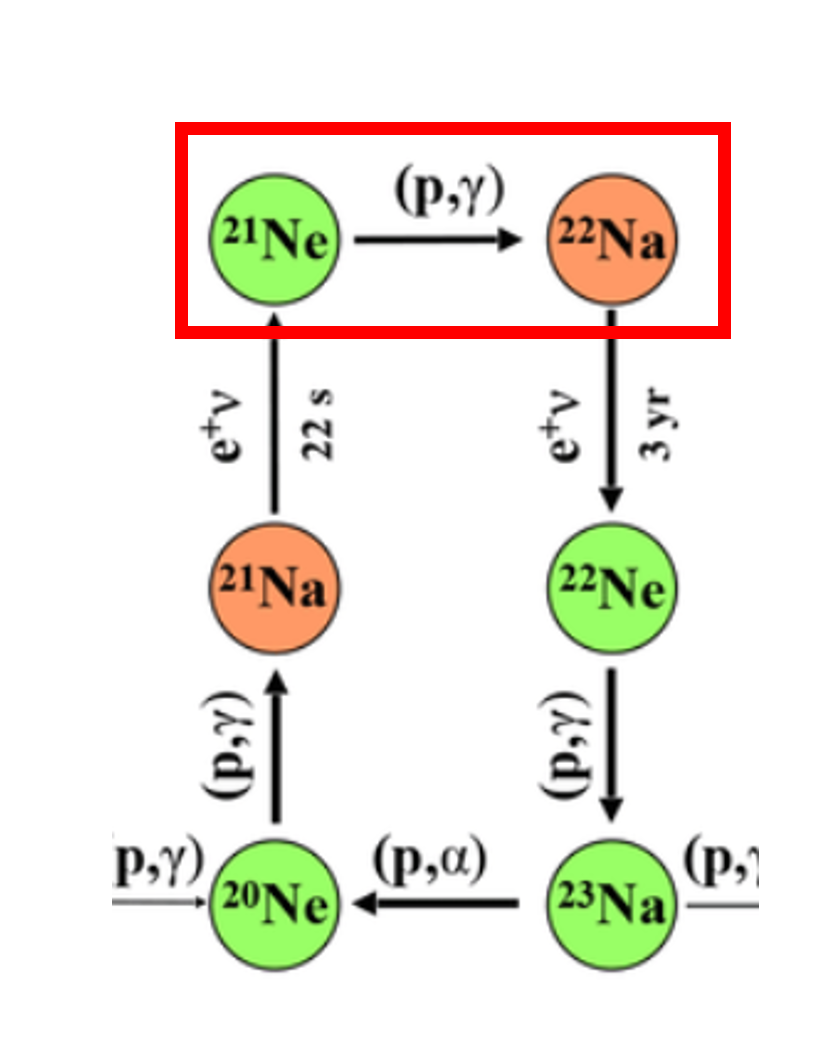
\includegraphics[width=5cm]{nena.png}
    \caption{Figure from \cite{nena}. Shown is the Neon-Sodium component of the Carbon-Nitrogen-Oxygen network with the \reac highlighted with the red box.}
    \label{fig:Nena}
\end{figure}

    When a star's core temperature reaches a critical threshold, thermonuclear reactions ignite which convert hydrogen to helium.  The star now enters a period of hydro-static and thermal equilibrium.  The reactions in the core are part of either the proton-proton (pp) chain or the carbon-nitrogen-oxygen cycle(CNO) \cite{iliadis2015}.  The latter is initiated at a core temperature of $\sim$15MK, which has the effect of activating the \textit{NeNa} (Neon-Sodium) cycle \cite{fowler1956}.  This is what drives the synthesis of elements between $^{20}$Ne and $^{24}$Mg.  There are particular stellar environments where it is active; the one of particular interest in \textit{classical novae}.  

    Classical novae are stellar phenomena that take place within close binary star systems, where a low-mass star transfers hydrogen-rich matter to a companion white dwarf. This matter forms an accretion disk around the white dwarf, gradually spiraling inwards and accumulating on its surface. Over time, the intense gravity of the white dwarf compresses this material, heating it up until a point where the dense bottom layer triggers a thermonuclear runaway, leading to a powerful explosion. This process is fueled by the rapid hydrogen to helium fusion via the CNO cycle, significantly increasing the system's luminosity—by a factor of about 10,000—and ejecting a substantial amount of matter into space at high velocities. Classical novae do not obliterate the white dwarf unlike supernovae, and can recur over tens to hundreds of thousands of years. With $\sim$ 35 occurrences annually in our Galaxy, classical novae are far more common than supernovae, highlighting a recurrent cycle of cosmic rebirth amidst the vast celestial expanse \cite{iliadis2015, boeltzig2016, masha2021}.

    At the energies of these classical novae, the cross section of $^{21}$Ne(p,$\gamma)^{22}$Na is comprised of resonances with high uncertainties \cite{chiara}. 

\subsection{$^{21}$Ne(p,$\gamma)^{22}$Na reaction}\label{reaction}

    Several coupled reactions make up the \textit{NeNa} cycle as shown in \ref{fig:Nena}.  We analyze the $^{21}$Ne(p,$\gamma)^{22}$Na reaction in particular due to its production of $^{22}$Na, an unstable isotope of sodium which arises in novae as explained above.  As mentioned in the introduction, certain qualities of this reaction make it easier to detect via direct observation as opposed to others.  The positron emission from sodium-22 results in the emission of gamma rays, which, coupled with its relatively long half-life of 2.6 years, provides a stable and detectable source of signals, making it highly suitable for extended studies of \reac by facilitating continuous and precise measurements of resonance strengths and reaction rates.  
    
    This reaction has $Q_{\text{value}}$ = 6739 keV, the positive value representing its exothermic quality \cite{krane1988}.  We arrive at an excited state of $^{22}$Na via an input resonance energy which will be explained in following sections.  This input energy, however, must be converted from the LAB frame to the COM frame (the center-of-mass frame for the particles).  This is done as follows,

    \[E_{\text{com}} = E_{\text{lab}} * \frac{M_{\text{T}}}{M_{\text{T}} + M_{\text{P}}},\]

    in which $M_T$ is the mass number of the target particle and $M_P$ is the mass number of the accelerator beam particle.  This is then added to the the $Q_{\text{value}}$ to identify the excitation energy $E_{\text{x}}$ for a given $E_{\text{p}}$, the energy input from the accelerator beam.  The reaction rate for the \reac is mainly due to the resonance strengths of the $E_{\text{p}}$=126 keV and $E_{\text{p}}$=272 keV resonances.  There are three others that have weaker contributions due mainly to lower resonance strengths, $E_{\text{p}}$=271, 290, and 352 keV \cite{GORRES1983372}.  It is worth noting, however, that the 126 keV resonance also has a low resonance strength, but its contribution is significant due to its low resonance energy $E$.  This can be numerically understood from the equation in section \ref{therm}.  For this report, the analysis will be for the 271 keV resonance. 

    Upon reaching an excited state, the $^{22}$Na isotope must decay to its ground state.  The transitions from the excited state to any level below it are called primary gammas, with the remainder called secondary gammas.  Each transition has a certain probability of occurring, known as a branching ratio.  These details are pictured in fig. \ref{fig:reac}.  

    \begin{figure}[H]
        \centering
        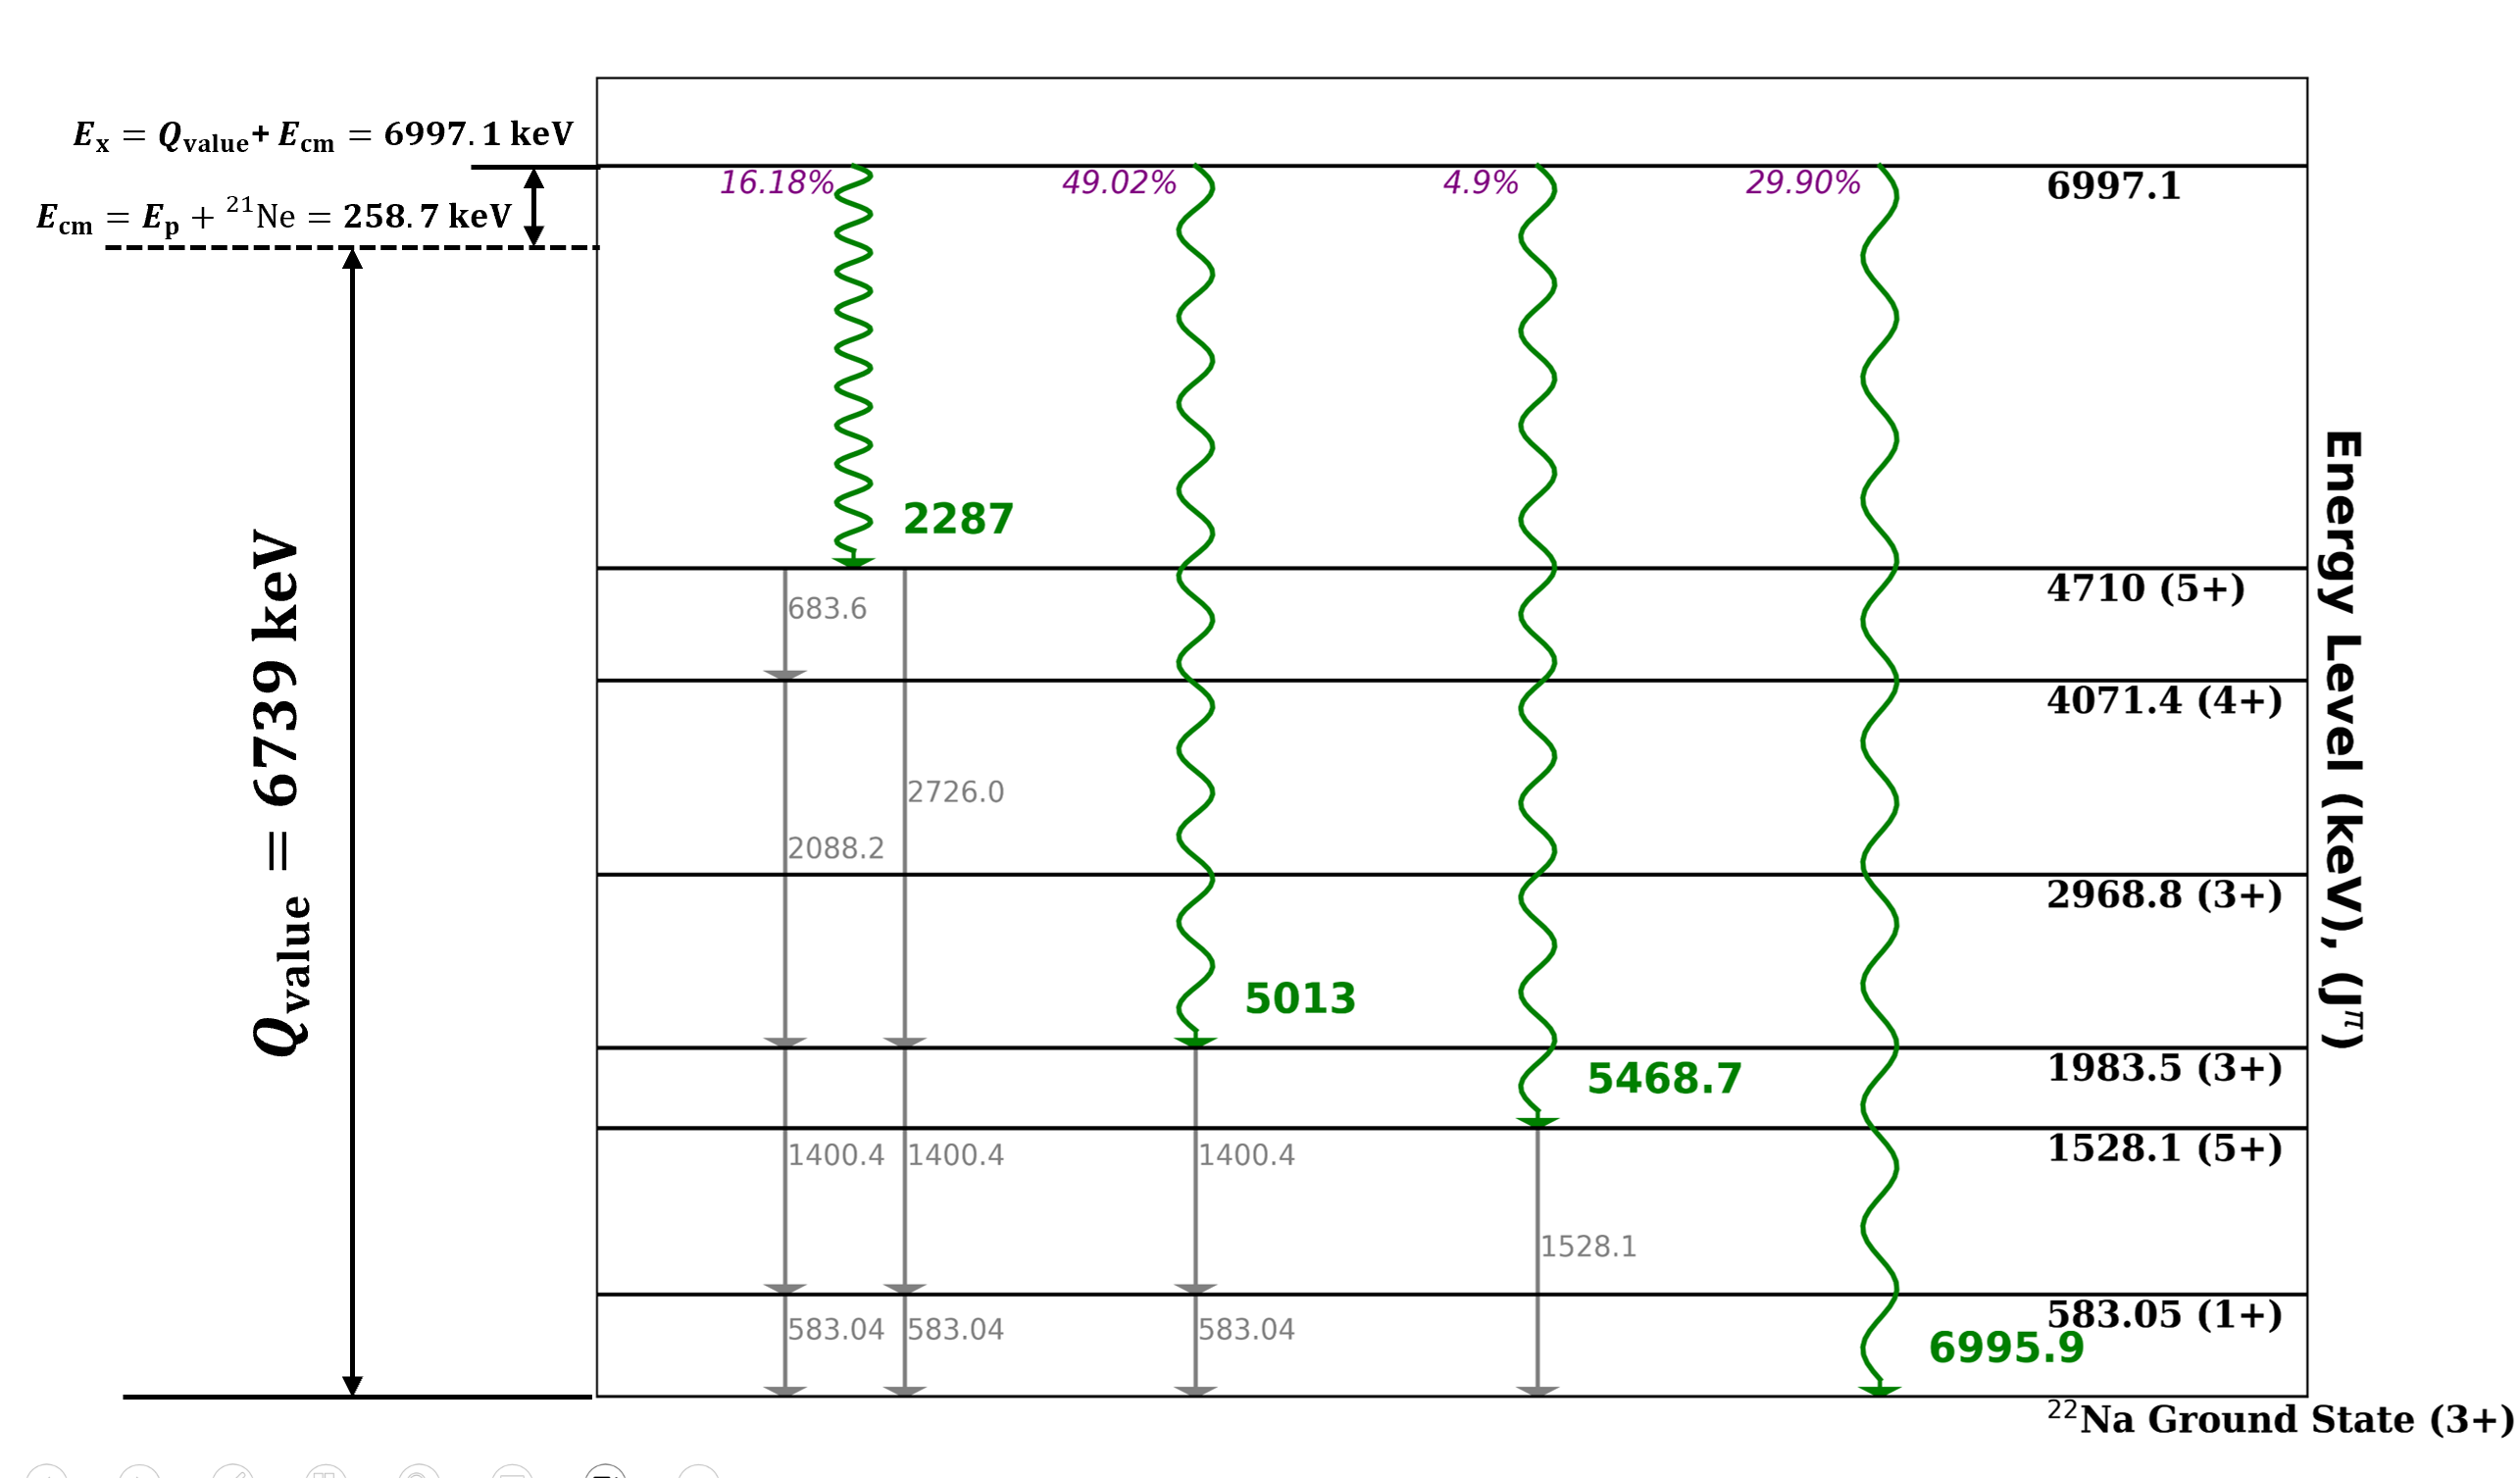
\includegraphics[width=15cm]{reac.png}
        \caption{Decay scheme for 271 keV resonance.  The arrival at the excited state is shown on the left side. 
 The diagram has four primary gammas shown in bold green.  The branching ratios are the values in purple.  The secondary gammas are the grey transition arrows.  The respective energy levels and $J^{\pi}$ are on the right side. Data from \cite{NNDCNuDat22Na}.}
        \label{fig:reac}
    \end{figure}

 
\section{Experimental Setup - LUNA}\label{luna}

In studies of stellar evolution, the relevant temperatures range from 20 to 100*10$^6$K, which corresponds to energies of 10–50 keV, depending on the precise reaction of interest \cite{Broggini2010}. At these energies, reactions induced by a charged particle such as \reac will have small cross sections, or essentially a low probability of occurring. Consequently, distinguishing the signals of interest from the background is most effectively done deep underground where interference from cosmic rays is reduced. 

The LUNA collaboration utilizes the low-background conditions offered by the subterranean laboratory beneath Italy's Gran Sasso Mountain (LNGS) to conduct direct measurements at astrophysical energies pertinent to their research. The overhead rock, with a thickness of 1400 meters, markedly diminishes cosmic interference: the muon flux decreases by a factor of one million, and the neutron flux by a factor of one thousand relative to levels found at the Earth’s surface \cite{Bemmerer2005}.

\subsection{Experimental Setup overview}

The central component to inducing the reaction at the LUNA facility is a proton beam, generated from a high-precision electrostatic accelerator (LUNA II 400 kV accelerator) \cite{FORMICOLA2003609}. This system ensures exceptional energy stability crucial for accurate cross-section measurements. The proton beam, created through ionization in a controlled gas mixture, is carefully directed to target setups via a  beam line, incorporating analyzing magnets and apertures for precise focusing. This setup, allowing for prolonged and unattended operation, is pivotal for investigating nuclear reactions under stellar-like conditions.

Shown in \ref{fig:luna_setup}, is the chamber which the beam enters centered upon the calorimeter. In order to study the \reac, we use two High-Purity Germanium Detectors (HPGe 1$\&$2), described later in \ref{HPGE}.  These generate the gamma-ray spectra that allow us to study different resonances.  Furthermore, a calorimeter is used for measurement of the beam intensity.  This component is essential in order to quantify the total energy and power output.  The entire chamber is filled with the Neon gas, notably without a dedicated entrance window.  This choice avoids various issues that could arise in relation to energy loss \cite{chiara}. Finally, lead bricks comprise a thick shielding which, in combination with being underground, serve to eliminated background effects and interference as much as possible.  In the following two sections we will go over the experimental parameters in detail of the proton beam and the gas target.  



\begin{figure}[h]
    \centering
    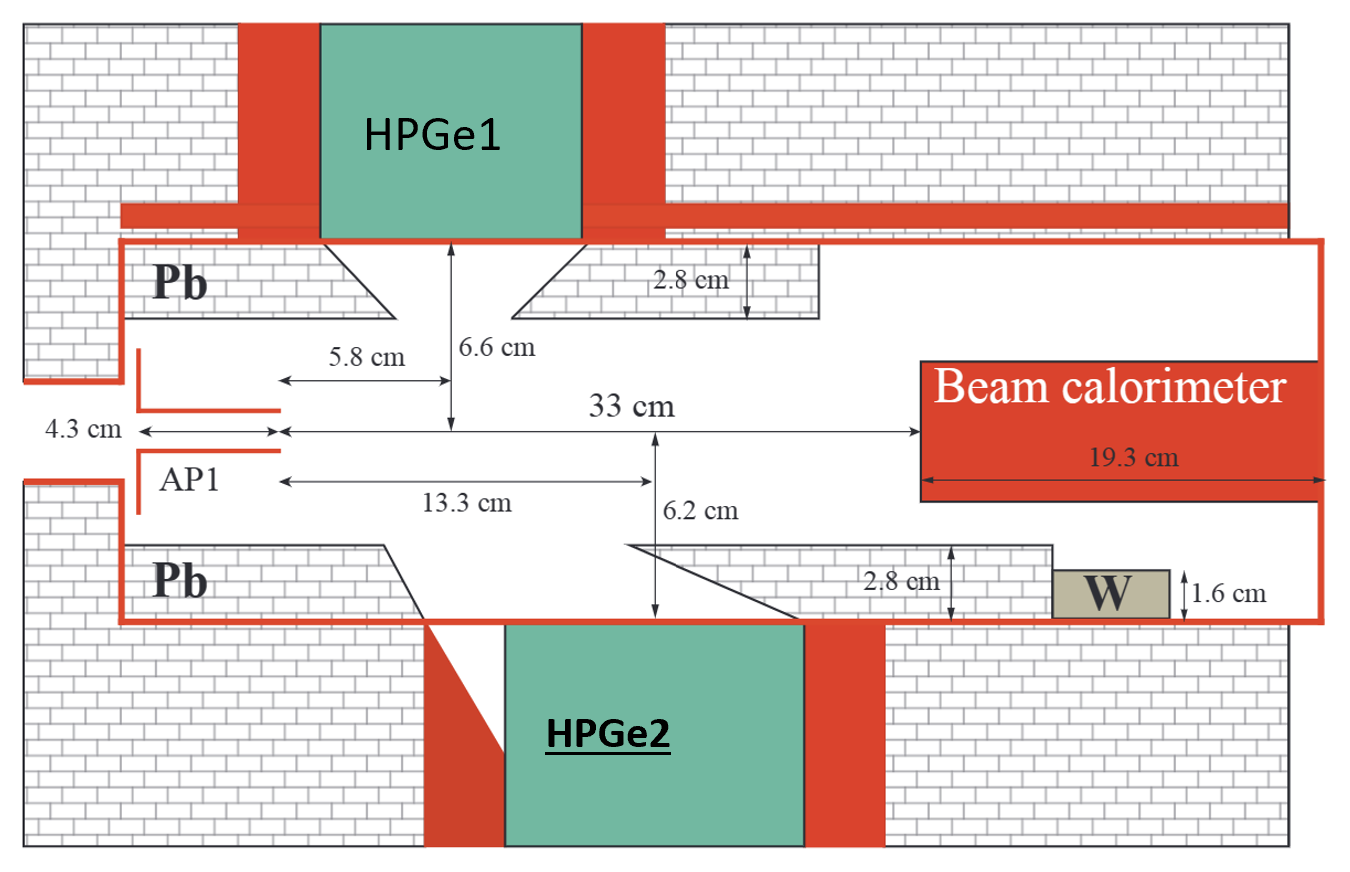
\includegraphics{luna_setip.png}
    \caption{Figure from \cite{cavanna2015}.  The setup is surrounded by lead bricks. The green items indicate the HPGe, with the bold HPGe2 being the detector from which the data analysed in the report is from. The beam current is measured by the beam calorimeter.  The item marked W is a tungsten disk, and AP1 is the collimator. Only HPGe2 and the calorimeter are directly relevant to the analysis in this report.}
    \label{fig:luna_setup}
\end{figure}


\subsubsection{Proton Beam}

The LUNA II accelerator features a power supply situated within the accelerator tank, providing the high voltage necessary for ion acceleration. Along with this is a radio-frequency ion source mounted directly on the accelerator tube, capable of continuous operation for approximately 40 days before necessitating replacement \cite{chiara}.

Capable of delivering high beam currents up to 1 mA for hydrogen (with a purity of 75\%) and up to 500 $\mu$A for helium, the LUNA II system significantly enhances experimental throughput. This high beam current is instrumental in augmenting the statistical accuracy of experiments focused on reactions with exceedingly low cross sections, as mentioned previously \cite{chiara}.


\textbf{Calibration and Beam Energy}


To analyze reactions with multiple resonances, selecting the beam energy involves a series of strategic decisions. Mentioned in \ref{reaction}, there are five resonances for the \reac, and we will analyse the 271 keV resonance for this report, so we must select a beam energy that sufficiently reaches the desired resonances after losing energy due to interactions with the gas ions (more on this in \ref{energy_loss}). Overall, practical adjustments for energy loss in the target, alongside experimental objectives—whether to measure cross-sections at peak resonances or to map the excitation function across a range of energies—further refine this selection. Ultimately, the chosen energy must account for the need to clearly resolve each resonance while accommodating the technical capabilities of the experimental setup and the specific goals of the study, ensuring accurate and meaningful results.

The calibration of the accelerator was performed using the $^{12}\text{C}(p,\gamma)^{13}\text{N}$ proton capture reaction, further validated through resonant reactions on $^{23}\text{Na}$, $^{25}\text{Mg}$, and $^{26}\text{Mg}$. These reactions also served to find the beam's energy spread, found to be less than 100 eV \cite{FORMICOLA2003609}. The calibration curve is described as a linear function of the sum of the terminal high voltage (TV) and the probe voltage (PV) of the ion source, mathematically represented as:

\begin{equation}
E_p = (0.9933 \pm 0.0002) \, \text{keV/kV} \cdot (TV + PV) - (0.41 \pm 0.05) \, \text{keV}
\end{equation}

This ensures that the uncertainty on the proton beam energy is maintained at 0.3 keV, with beam stability surpassing 5 eV/h, exemplifying the high precision achievable with the LUNA II facility \cite{FORMICOLA2003609}.


\subsubsection{Gas Target}

The investigation of the \reac is conducted in two phases, employing different gas compositions . The initial phase uses natural neon with isotopic proportions of 90.48\% \(^{20}\text{Ne}\), 0.27\% \(^{21}\text{Ne}\), and 9.25\% \(^{22}\text{Ne}\). Due to the low natural occurrence of \(^{21}\text{Ne}\), the second phase utilizes neon gas enriched to 59\% \(^{21}\text{Ne}\). Both phases leverage a windowless gas target in a recirculating configuration. While the initial phase examines two resonances within natural neon, the focus of this thesis is on the enriched \(^{21}\text{Ne}\) gas utilized in the second phase.

The use of a gas target presents several advantages in the context of nuclear astrophysics experiments. A key benefit is the gas's resilience to degradation under prolonged ion beam exposure, crucial for maintaining target stability during intensive ion beam irradiation. Moreover, gas targets can achieve high isotopic purity, reducing background noise from contaminants \cite{Best2016UndergroundNA}.

An important feature of gas targets is the ability to adjust the target thickness by altering the gas pressure. This flexibility facilitates the customization of experimental conditions to specific research needs. Accurate determination of gas density is essential, considering its dependence on temperature and pressure, including variations caused by the beam's heating effect.  More detail about the determination of gas density will come in \ref{target_density}.  Additionally, as mentioned previously, the choice of a windowless target is primarily driven by the need to minimize energy loss and to ensure more accurate measurements, reflecting the careful planning and precise execution required for these experiments.


\subsection{High-Purity Germanium Detectors}\label{HPGE}

The setup for this reaction includes two High-Purity Germanium detectors (HPGe), placed 90$^\circ$(HPGe1) and 55$^\circ$(HPGe2) with respect to the beam direction.  These have relative efficiencies of 90\% and 130\% with respect to a NaI scintillation detector and $^{60}$Co sample configuration \cite{chiara}.  This configuration enhances the data quality in a number of different ways: 1) the different angles allow for the detection of gamma rays emitted at specific angles relative to the beam direction, enabling the measurement of branching ratios for the resonance decay. Since various resonant states can decay by emitting gamma rays in different directions, having two detectors at distinct angles helps in deconvoluting these paths; 2) using multiple detectors reduces the systematic errors that could arise from the alignment, electronic response, or efficiency variances in a single detector setup, such that if one detector were to malfunction or display anomalous results, the second detector serves as a check against such errors; 3) the offset positions of the detectors help in covering a wider solid angle overall, which ensures that more of the emitted gamma rays are detected, leading to a higher efficiency for detecting the resonance decays.  This report will only analyse a single detector, HPGe2, but in general one must factor in the data from multiple detectors for best results.

As for the specific choice of HPGe's as opposed to other types of detectors, the energy resolution is highest.  In cases where a reaction with multiple resonances produces several gammas, it is essential that the peaks are distinguised as much as possible. A comparison between HPGe and NaI detectors is shown in \ref{fig:detector_compare}.

\begin{figure}[h!]
    \centering
    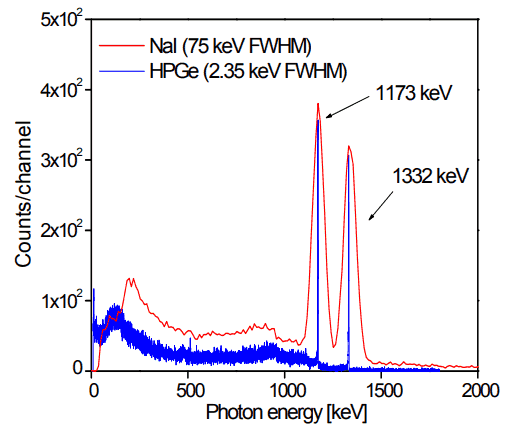
\includegraphics[width=10cm]{detector_compare.png}
    \caption{Figure from \cite{ByunLectureNotes}. Shows a resolution comparisison between NaI and HPGe detectors for a colbalt-60 source.}
    \label{fig:detector_compare}
\end{figure}



\subsection{Calorimeter}\label{calorimeter}

Due to the charge state fluctuations of the low energy ions and the secondary electrons produced by ionization as the ion beam passes through the gas target, traditional methods like the Faraday cup are not feasible \cite{cavanna2015, chiara}. These effects prevent an accurate measurement of the beam current by direct electrical means.

To resolve this, a beam calorimeter was integrated into the system. This device quantifies the power deposited by the beam instead of measuring the current directly. The calorimeter, designed with a copper construction, operates on the principle of maintaining a constant temperature gradient between two thermally coupled sides, known as the hot side and the cold side. The cold side is maintained at 0°C using a cooling system, while the hot side, functioning as the beam stopper, is held at a steady temperature of 70°C. This temperature regulation is achieved through a combination of heat from the ion beam impact and auxiliary heating resistors.  The heat load on the hot side has two sources: the ion beam itself and the heat provided by the resistors \cite{masha2021}. 

The intensity of the beam is derived from the power deposited by the beam on the calorimeter, a critical quantity for experiments that require precise beam characterization. The calculation of the beam intensity \( I \) is facilitated by the equation:

\begin{equation}\label{int}
I = \frac{W_0 - W_{\text{beam}}}{E_{\text{beam}} - \Delta E_{\text{beam}}} \cdot e
\end{equation}

where \( W_0 \) is the power supplied by the resistors when the ion beam is off, providing a baseline measurement of the power required to maintain the calorimeter at operational temperatures. \( W_{\text{beam}} \) represents the power supplied by the resistors when the ion beam is on, typically lower than \( W_0 \) due to the additional heat contributed by the beam. The difference between these two, \( W_{\text{calo}} = W_0 - W_{\text{beam}} \), is thus the power attributable to the beam. The term \( E_{\text{beam}} - \Delta E_{\text{beam}} \) accounts for the beam's energy after traversing the gas target, reflecting the initial energy minus any losses encountered en route. Accurate readings of temperature and power adjustments are recorded by a data acquisition system, which, alongside the known properties of the calorimeter, allows for precise determination of the beam's intensity.

\textbf{Calorimeter Calibration}

Calibration of the calorimeter is a critical process to ensure accurate correlation between calorimetric power, \(W_{\text{calo}}\), and electrical power, \(W_{\text{el}}\). This step is necessary to correct the beam intensity as presented in eq. \ref{int}. The calibration process validates the expectation that \(W_{\text{el}} = C \cdot W_{\text{calo}}\) with the calibration constant \(C\) close to 1.

A calibration performed in \cite{masha2021} in October 2020 was used for the analysis in this report. Multiple runs were recorded to capture consistent \(W_0\) values, the power supplied by the resistors in absence of the beam. The calibration revealed a linear relationship between \(W_{\text{el}}\) and \(W_{\text{calo}}\), expressed as:

\begin{equation}
W_{\text{el}} = m \cdot W_{\text{calo}} + q
\end{equation}

with the resulting slope \(m = 0.986 \pm 0.002\) and offset \(q = -0.2 \pm 0.1\) W.




\section{Data Analysis}\label{data}
\subsection{Overview - {\textit{Thick-Target}} approach}\label{approach}

To present our goal again, we aim to obtain the resonance strength $\omega\gamma$ for the $E_{\text{p}}$ = 271 keV resonance.  There exists different ways to represent the yield Y of a reaction based on the width $\Gamma$ of the resonance.  To summarize, if the target thickness (a Neon gas in our case) is significantly greater than the resonance width $\Gamma$,essentially cases where all projectiles within the beam energy distribution contribute to the resonance yield, we use the so called \textit{Thick-target} approach from \cite{RolfsRodney1988}.  We effectively assume the target is infinitely thick, denoting the yield as $Y_{\infty}$, which is proportional to $\omega\gamma$ by the following, 

\begin{equation}
Y_{\infty} = \frac{\lambda^2}{2} \omega\gamma \left( \frac{m + m_{\text{t}}}{m_{\text{t}}} \right) \frac{1}{\varepsilon_{\text{eff}}}
\end{equation}
where \( \lambda \) is the de Broglie wavelength associated with the resonance condition in the reaction and is proportional to the resonance energy \( E_r \). The resonance strength is denoted by \( \omega\gamma \). \( m_{\text{t}} \) represents the mass of the target nuclei, in this context \( ^{21}\text{Ne} \), and \( m \) is the mass of the projectile, a proton with mass \( m_{\text{p}} \). The effective stopping power \( \varepsilon_{\text{eff}} \) is calculated at the resonance energy, representing the energy loss of the projectile per unit path length within the target material. This stopping power is a vital parameter, as it influences the reaction yield by determining how much energy the projectile loses as it penetrates the target, which in turn affects the number of reactions that can occur.

Therefore, the yield parameter is what we aim to calculate, expressed as number of reactions per projectile.  This is done by obtaining a total number of reaction counts in the spectrum, and normalizing it to the integrated charge:

\begin{equation}
    Y = \frac{N_{\text{counts}}}{Q}.
\end{equation}

In the next sections, we will 1) use the Gamma-ray spectrum from HPGe2 to identify the resonance peaks of interest; 2) calculate the area and apply corrections for efficiency to obtain the total number of reactions.  Following this we will calculated charge using the experimentally measured data for power and energy.  We will also consider factors of the target density and stopping power on energy loss.

\subsection{Gamma-ray spectrum analysis}

A given gamma-ray spectrum may resemble an overlapping combination of the features shown in \ref{fig:combined}. Key features observed in the spectrum include:

\begin{enumerate}
    \item \textbf{Photo-electric peak:} The distinct peak representing the full absorption of gamma-ray energy via photoelectric interaction.
    \item \textbf{Compton Edge:} The sharp cutoff in the spectrum, marking the maximum energy transferred to an electron during Compton scattering.
    \item \textbf{Backscatter Peak:} A lower energy peak resulting from gamma rays scattering off the detector shielding back into the detector.
    \item \textbf{Single Escape Peak:} A peak reduced by 511 keV from the original energy, indicative of a positron escaping the detector after pair production.
    \item \textbf{Double Escape Peak:} A peak reduced by 1022 keV when both particles from pair production escape the detector.
\end{enumerate}

Each feature provides insights into the interaction of gamma rays with the detector and contributes to the determination of the source's characteristics.  For the purpose of obtaining the total number of reactions, $N_{\text{counts}}$, we will take the area under the photo-electric peaks of the primary gamma transitions identified in the spectrum.


\begin{figure}[H]
    \centering
    \begin{subfigure}{0.49\textwidth}
    \centering
    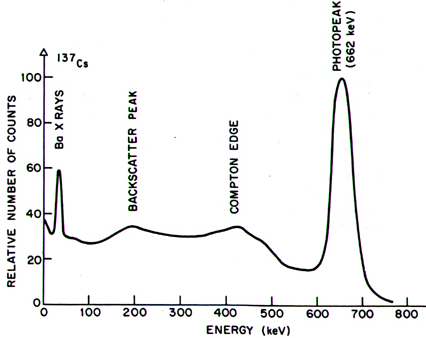
\includegraphics[width = \textwidth]{grs1.png}
    \caption{Shows photopeak, compton edge, and backscatter in gamma-ray spectrum.}
    \label{fig:grs1}
    \end{subfigure}
    \begin{subfigure}{0.49\textwidth}
    \centering
    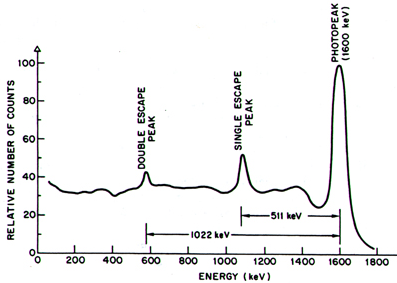
\includegraphics[width = \textwidth]{grs2.png}
    \caption{Shows how escape peaks can appear on a gamma-ray spectrum.}
    \label{fig:grs2}
    \end{subfigure}
    \caption{Figures from \cite{CrosthwaitPulseAnalysis}. Features found in a gamma-ray spectrum.}
    \label{fig:combined}
\end{figure}



\subsubsection{Energy calibration}

Due to the nature of the data acquisition system of the HPGe detectors used, we obtain the spectra in counts vs. channel number.  We must convert a given spectrum to counts vs. energy by taking known sources and applying calibration constants.  This process is repeated periodically when there is a noticeable shift in the spectrum of where an expected reaction should be and where it appears.  At times, a dedicated source is added such as $^{137}$Cs to produce a reaction. Alternatively, the ${}^{19}\text{F}(p,\alpha\gamma){}^{16}\text{O}$ reaction which occurs naturally in the target chamber serves as an effective source. Shown in \ref{calib_tab}, are the sources used and their respective energies.  In \ref{fig:uncalib}, the uncalibrated spectrum and the location of the calibration peaks is shown.  To obtain a precise mean, $\mu$, of each peak, a normalized Gaussian function is fitted to it.  More detail about this function will be in the following section as we begin to calculate areas, \ref{area}.

\begin{table}[ht]
\centering
\begin{tabular}{||c | c ||} 
 \hline
 Decay/Reaction & Energy (keV) \\ [0.5ex] 
 \hline\hline
 $\beta$+ emission & 511 \\ 
 \hline
 $^{22}$Na & 1274.5  \\
 \hline
 ${}^{19}\text{F}(p,\alpha\gamma){}^{16}\text{O}, \text{double escape peak}$ & 5108 \\
 \hline
 ${}^{19}\text{F}(p,\alpha\gamma){}^{16}\text{O}, \text{single escape peak}$ & 5619 \\
 \hline
 ${}^{19}\text{F}(p,\alpha\gamma){}^{16}\text{O}, \text{full energy peak}$ & 6130 \\ [1ex] 
 \hline
\end{tabular}
\caption{Calibration energies for various decays and reactions.}
\label{calib_tab}
\end{table}



\begin{figure}[h!]
    \centering
    \hspace*{-1.5cm}
    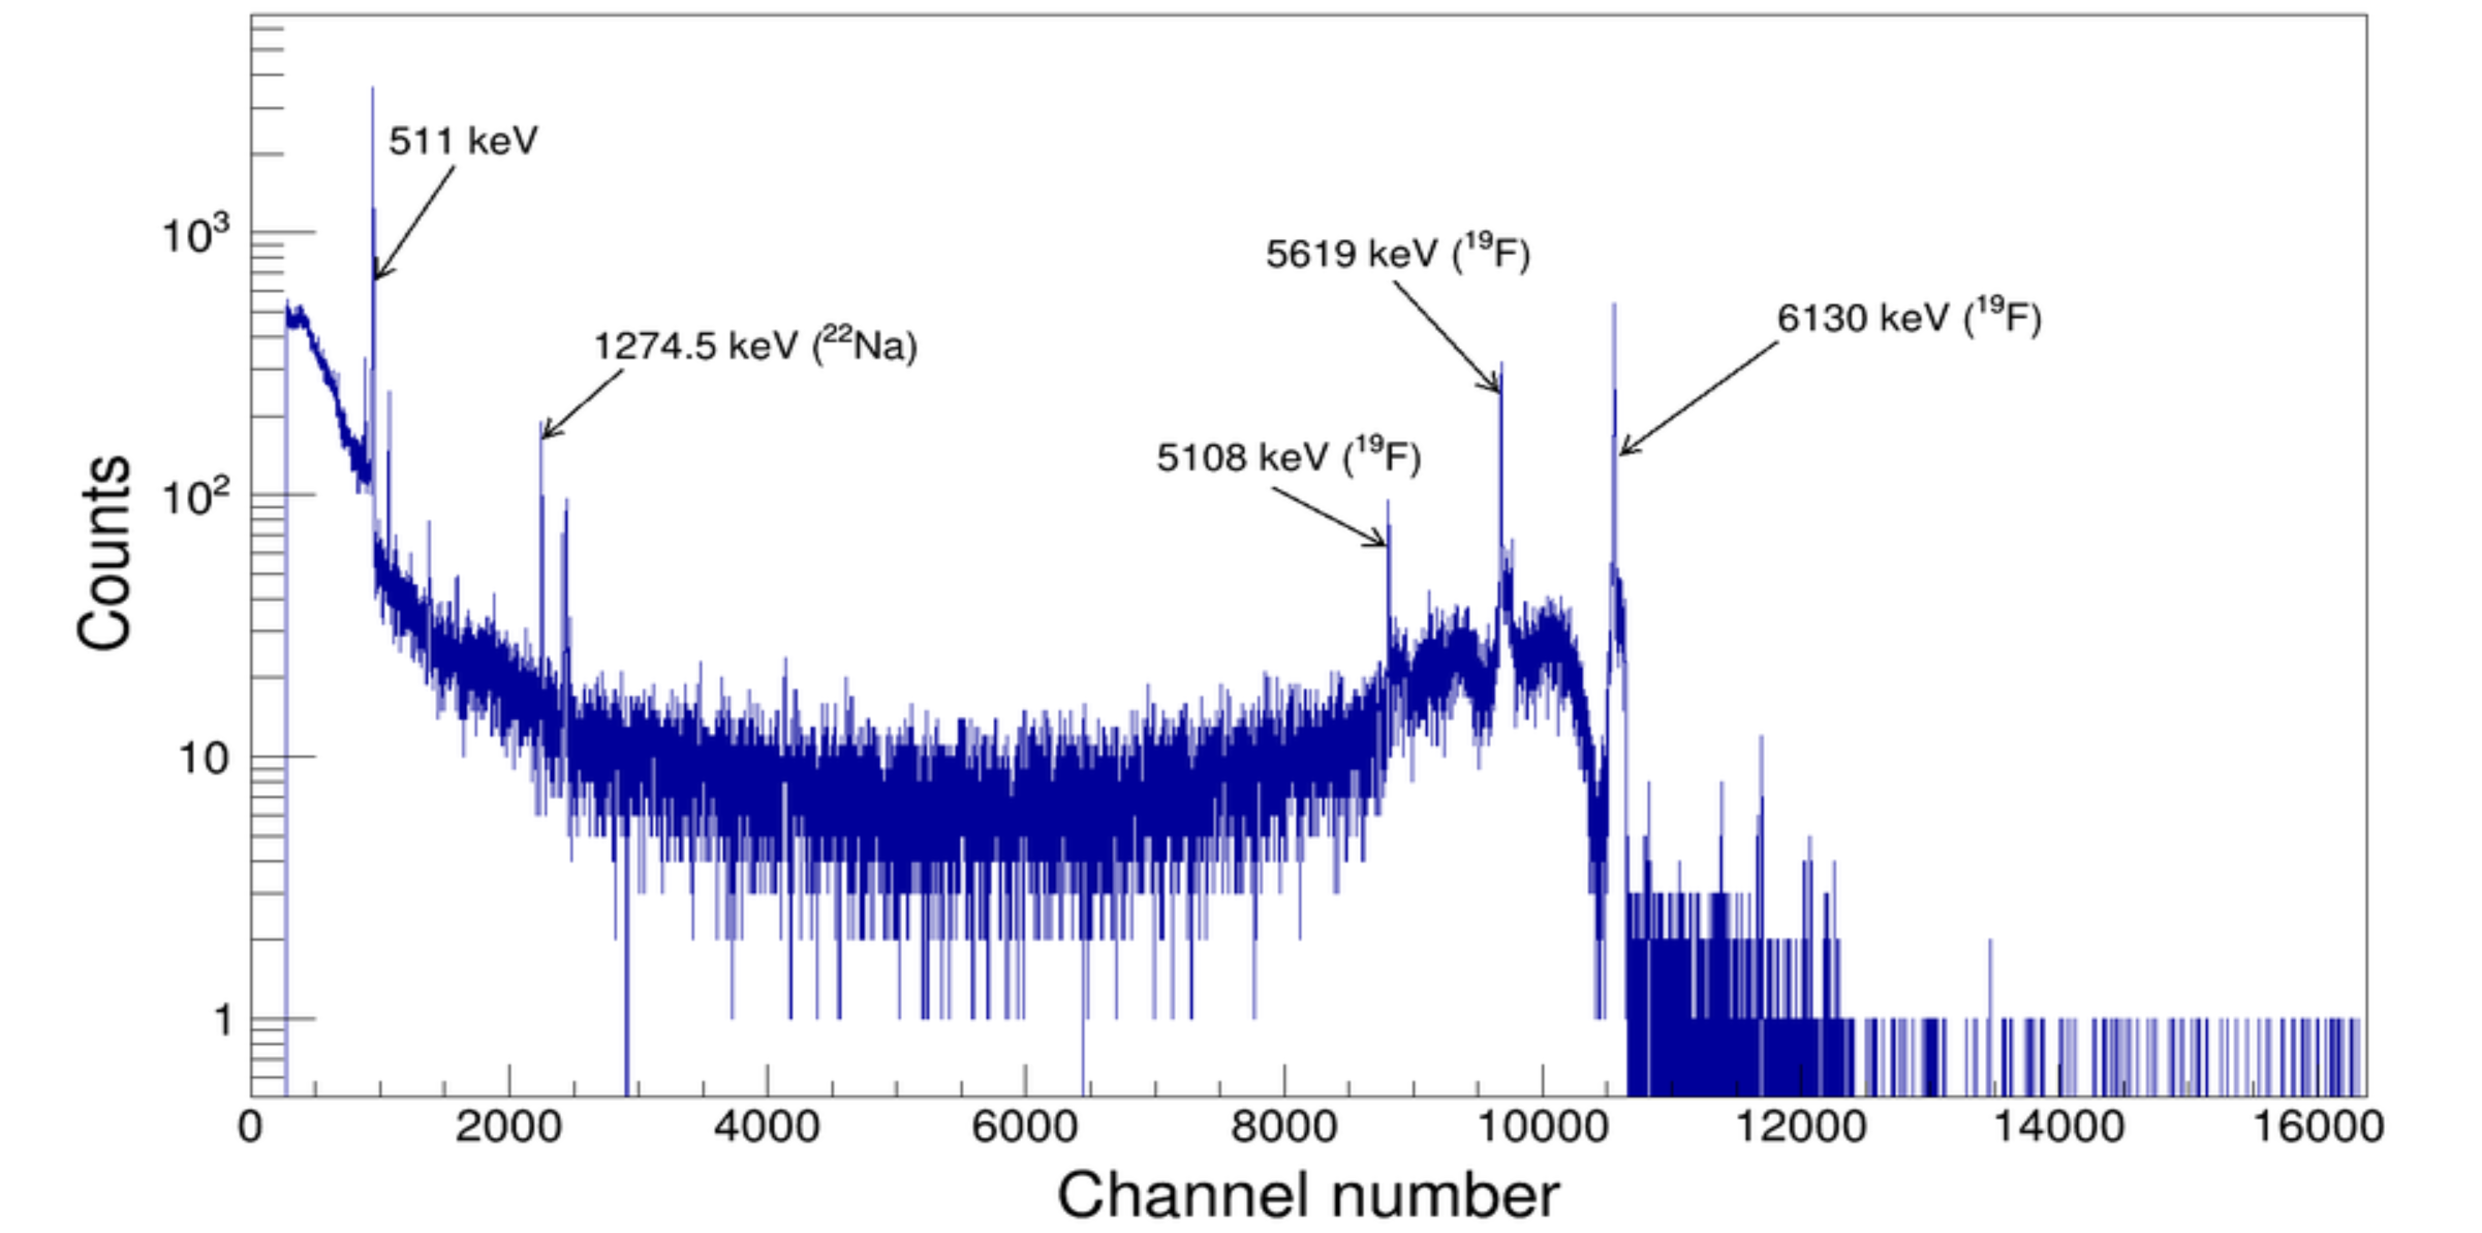
\includegraphics[width=18cm]{uncalib_spec.png}
    \caption{A gamma-ray spectrum taken with no target.  The highlighted peaks represent known reactions/decays used for calibration.}
    \label{fig:uncalib}
\end{figure}

\begin{figure}[H]
    \centering
    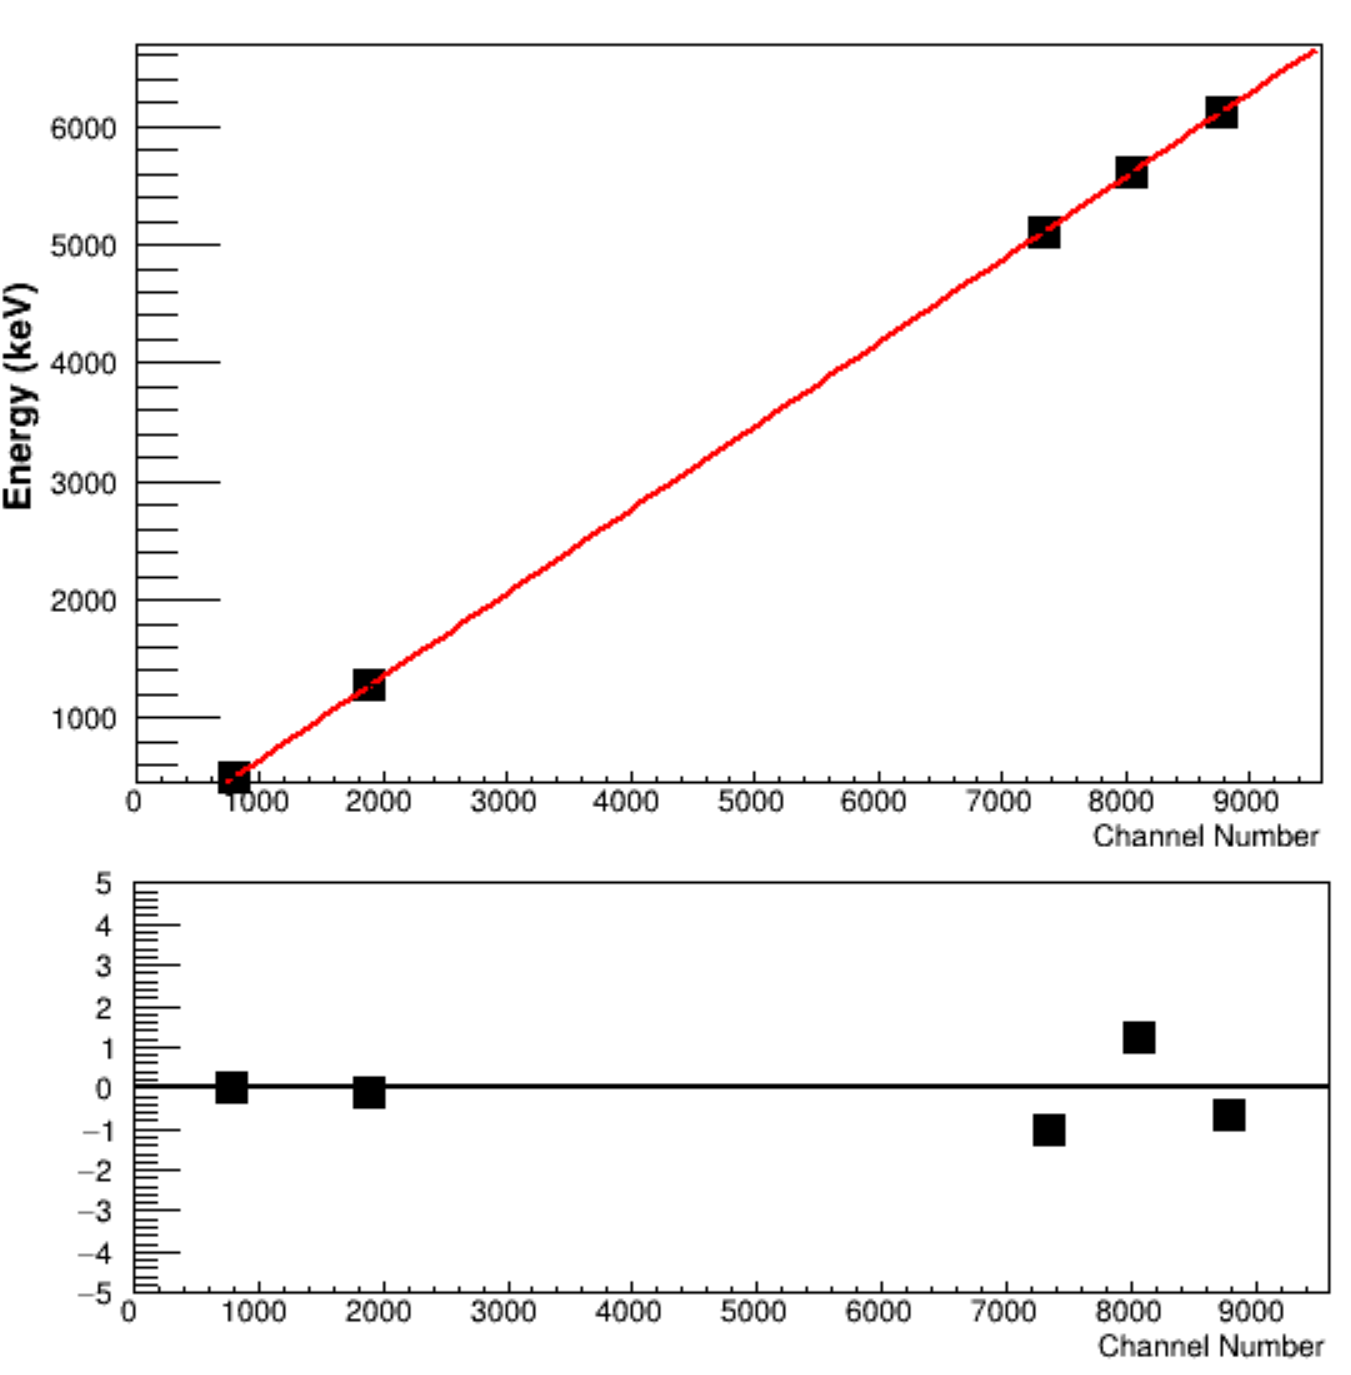
\includegraphics[width=8cm]{calib_fit.png}
    \caption{Linear calibration plot and residuals. Equation takes the form y[keV] = m[keV/channel]*channel + q[keV].  Fit produced 0.7037(1) +-49.2(8), with $r^2$=0.999998.  Residuals support that this is a sufficiently strong fit.}
    \label{fig:calib_fit}
\end{figure}

Pictured in \ref{calib_tab}, A linear fit is applied to the energies and channel numbers to obtain calibration constants m, $\frac{\text{keV}}{\text{channels}}$ and q, ${\text{keV}}$.  These were 0.7037 $\pm$ 0.0001 and -49.2 $\pm$ 0.8 respectively.  Now, the calibrated spectrum is produced with the location of the primary gammas highlighted, as shown in \ref{fig:calib_spec}.



\begin{figure}
    \centering
    \hspace*{-1.5cm}
    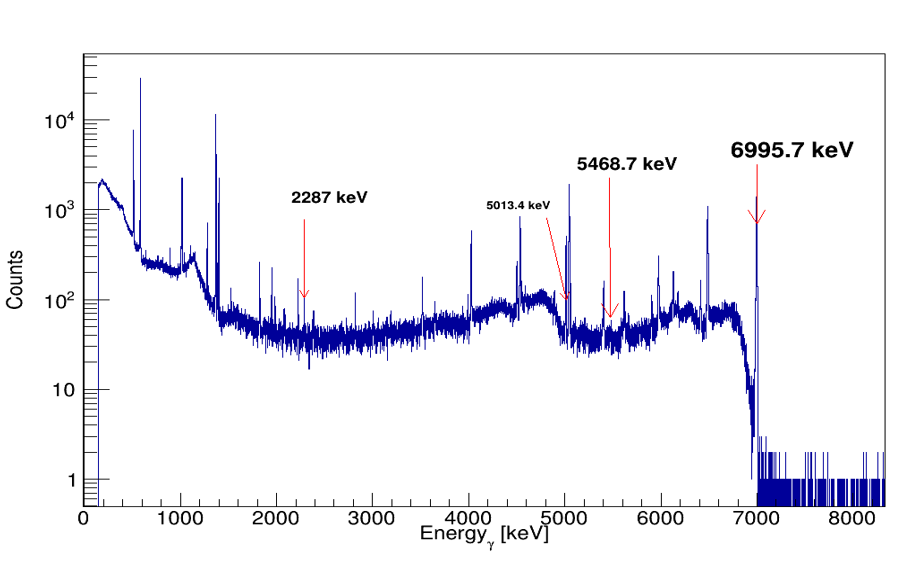
\includegraphics[width=16cm]{calib_spec.png}
    \caption{Calibrated spectrum with primary gammas highlighted by red arrows.}
    \label{fig:calib_spec}
\end{figure}



\subsubsection{Peak area calculation}\label{area}

 The primary challenge with calculating area of a peak is accurately subtracting the background contribution.  Two methods are generally employed to calculate this net area, the first by fitting a composite function consisting of a normalized Gaussian function and a first order polynomial: 

\begin{equation}
f(x) = \frac{A}{\sigma\sqrt{2\pi}} \exp\left(-\frac{(x-\mu)^2}{2\sigma^2}\right) + Bx + C
\end{equation}

where \( A \) signifies the total area under the Gaussian curve, \( \sigma \) is the standard deviation, \( \mu \) locates the center of the peak, the exponential function forms the Gaussian profile, \( B \) represents the slope of the first-order polynomial, and \( C \) is its y-intercept.  Depending on the quality of the peak, one may choose to use several Gaussians to perform the fitting.  In cases there the peak is non-symmetrical, a tail parameter $\lambda$ is added as follows, 

\begin{equation}
f(x) = \frac{A}{\sigma\sqrt{2\pi}} \exp\left(-\frac{(x-\mu)^2}{2\sigma^2}\right) \left[1 + \text{erf}\left(\lambda\frac{x-\mu}{\sigma\sqrt{2}}\right)\right]
\end{equation}


where $\text{erf}$ is the error function.  

Alternatively, there is the \textit{Covell Method}, also known as the \textit{Gilmore Method} \cite{gilmore2008}, which streamlines peak area calculation by first summing the counts within the peak limits to find the gross peak area \( G \), and then estimating the background \( B \) using adjacent channel counts. The process is represented by:

\[
G = \sum_{i=L}^{U} C_i, \quad B = n \cdot \frac{CL_{-1} + CU_{+1}}{2},
\]

where \( C_i \) denotes counts in channel \( i \), \( L \) and \( U \) define the peak boundaries, and \( n \) is the count of channels in the peak. The net peak area \( A \) is the gross area minus the background, \( A = G - B \). The measurement's uncertainty, \( var(A) \), is the sum of the variances of \( G \) and \( B \), crucial for precision in gamma-ray spectrometry. Table \ref{table:area_calc_comparison} summarizes the benefits/use-cases of each method.  Before deciding which method to employ let us observe the peaks in the spectrum.  

Recall that we have 4 primary gamma transitions for $E_{\text{p}}$ = 271 keV, so we would need to take the sum of the area for all of these to obtain the total number of reactions $N_{\text{counts}}$.  First, however, we recognize a couple of complications.  Table \ref{tab:nndc} shows that two transitions from the $E_{\text{x}}$ = 6997.1 keV are indistinguishably close to two found in $E_{\text{x}}$ = 6998.1 keV.  Furthermore, the 5468.7 keV transition has an intensity $I$ that is too low.  This value represents the relative probability of a transition as explained in section \ref{reaction}. In figure \ref{fig:other_pg}, this information is verified by observing the peaks in the spectrum itself.  

\begin{table}[H]
\centering
\begin{tabular}{||c|c|c||}
\hline
\textbf{E(level) (keV)} & \textbf{E($\gamma$) (keV)} & \textbf{I($\gamma$)} \\
\hline
6997.1 $\pm$ 4 & 2287 & 33 $\pm$ 4 \\
& \hl{5013.4} & 100 $\pm$ 6 \\
& \textbf{5468.7} & \textbf{10 $\pm$ 2} \\
& \hl{6995.9} & 61 $\pm$ 4 \\
\hline
6998.1 $\pm$ 4 & 1824 & 1.8 $\pm$ 4 \\
& 4028.7 & 8.4 $\pm$ 18 \\
& \hl{5014.4} & 11.8 $\pm$ 10 \\
& 5045.8 & 58 $\pm$ 4 \\
& 5060.5 & 3.4 $\pm$ 10 \\
& 6414.3 & 3.6 $\pm$ 8 \\
& \hl{6996.9} & 100 $\pm$ 4 \\
\hline
\end{tabular}
\caption{Data from \cite{NNDCNuDat22Na}. Highlighted values are the ones mixed between both resonances, bold values show the primary gamma with a low intensity I($\gamma$).}
\label{tab:nndc}
\end{table}

In fig. \ref{fig:plot}, we see the 2287 keV transition which is not mixed with any others, and is easy to discern from the background.  Furthermore, the background is shaped such that there is not a significant slope or additional peaks that would make it difficult to define.  For these reasons, the \textit{Covell Method} is a reasonable choice to find the area to utilize for the remainder of the calculations. Fig. \ref{fig:plot} also shows that generally these areas are within one error bar of each other.





\begin{figure}[H]
    \centering
    \hspace{-1.5}
    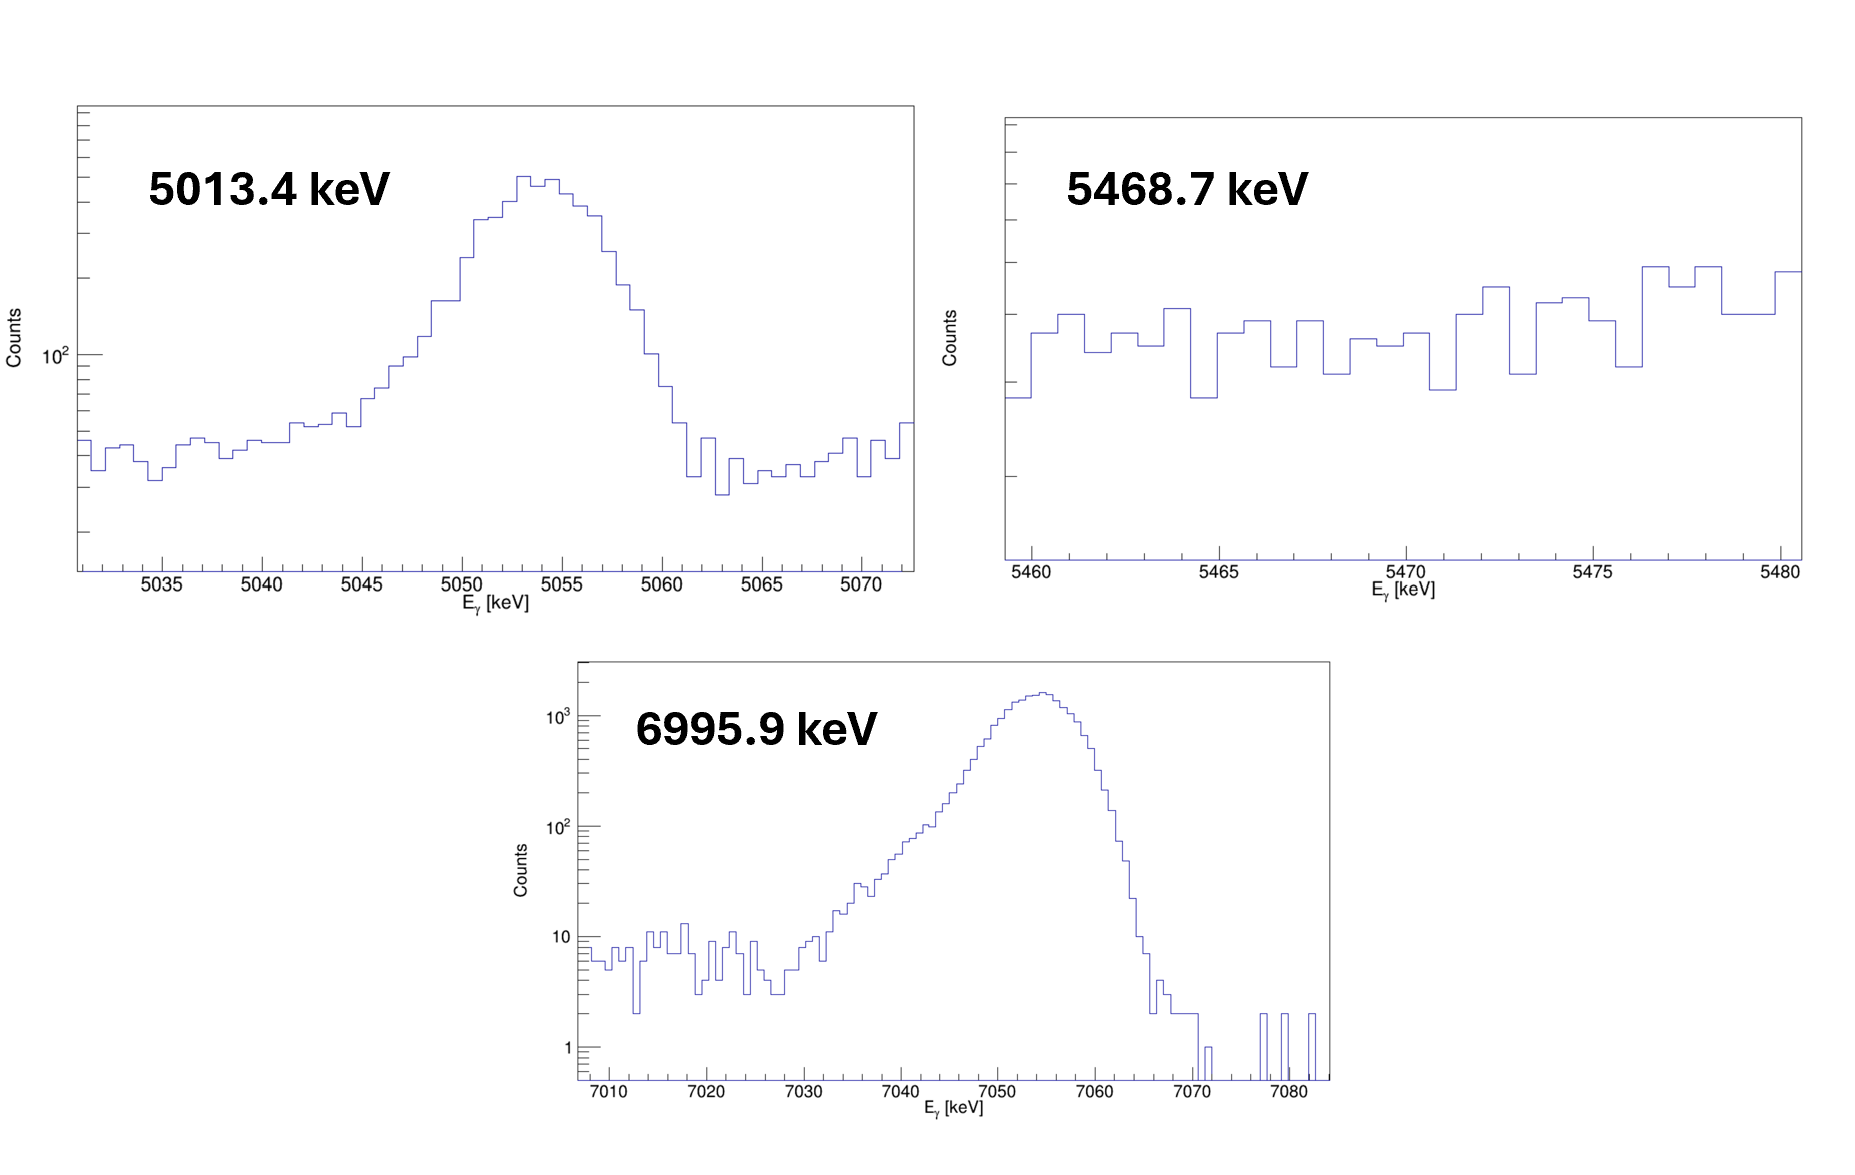
\includegraphics[width=16cm]{other_pg.png}
    \caption{Primary gamma peaks that could not have their area calculated easily. The 5013.4 and 6995.6 keV experience mixing from the 1 keV resonance above, and 5468.7 keV has too low of an intensity.}
    \label{fig:other_pg}
\end{figure}

\begin{table}[h]
\centering
\label{table:area_calc_comparison}
\begin{tabular}{||p{0.45\textwidth}|p{0.45\textwidth}||}
\hline
\textbf{Covell Method} & \textbf{Gaussian Fit} \\
\hline
1. Does not require curve fitting algorithms, making it straightforward and computationally simple. & 1. Provides a precise fit for well-defined, isolated peaks, resulting in accurate peak area estimation. \\
\hline
2. Effective for quick analysis when peaks are non-overlapping and background is relatively constant. & 2. Beneficial for complex spectra with overlapping peaks, as it can deconvolute and quantify each peak individually. \\
\hline
3. Suitable for spectra with a large number of peaks, allowing for rapid automated processing without sophisticated fitting procedures. & 3. Does not require a level, well-defined background. \\
\hline
\end{tabular}
\caption{Comparison of Area Calculation Methods in Gamma Spectrometry}
\end{table}


\begin{figure}[H]
    \centering
    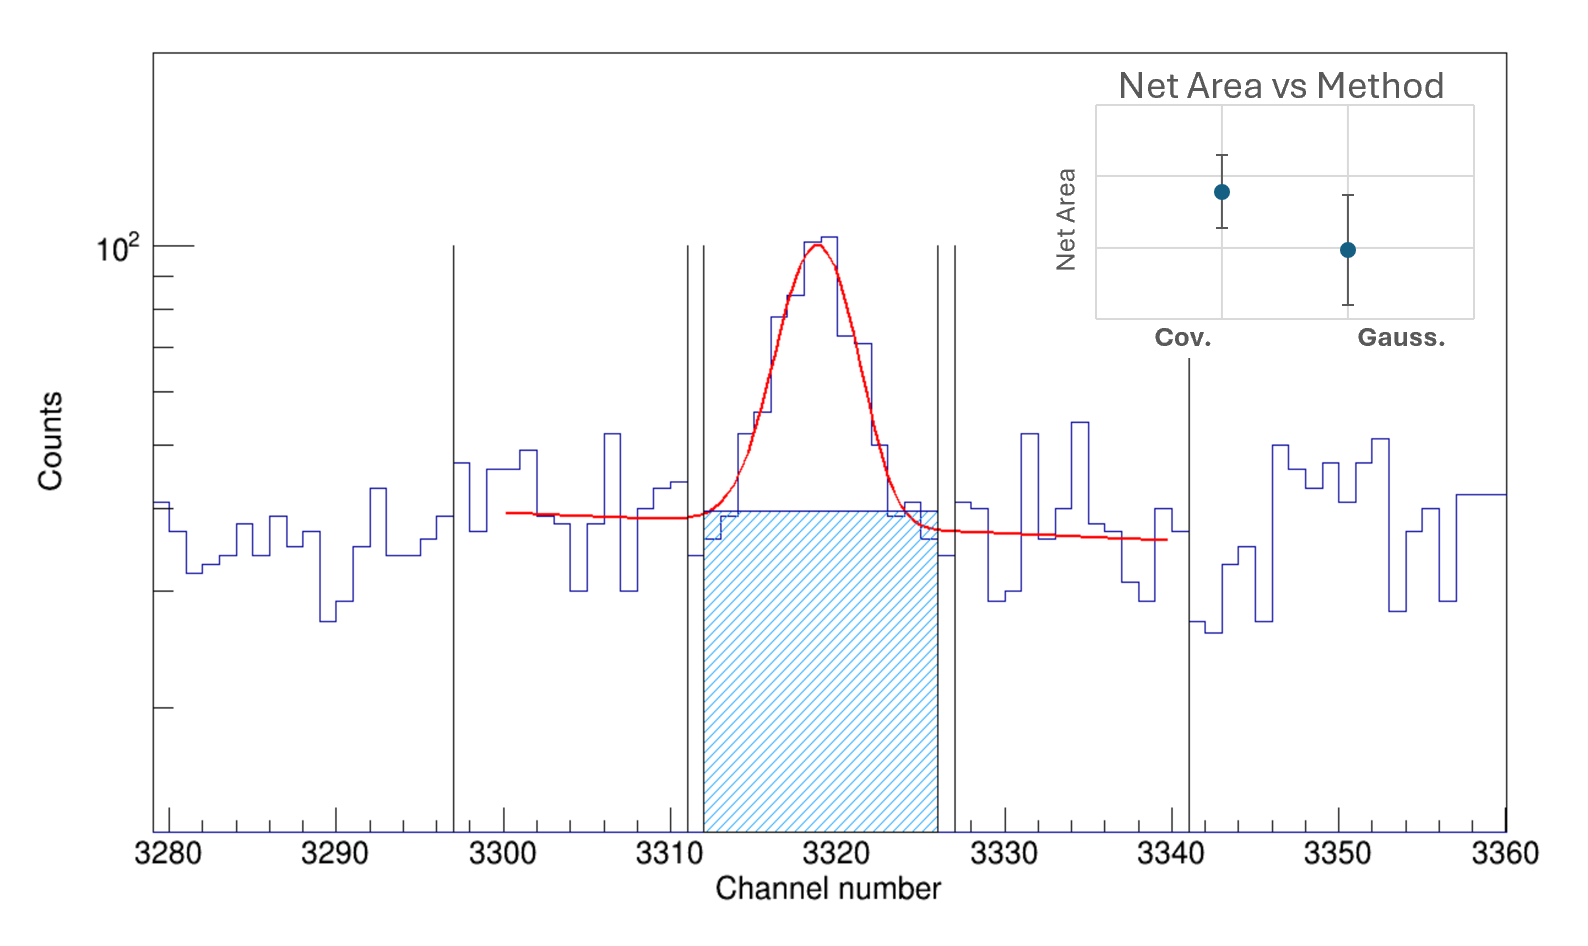
\includegraphics[width=16cm]{plot3.png}
    \caption{Normalised Gaussian fit applied to 2287 keV peak (no tail parameter $\lambda$ needed. Black lines surrounding peak mark the background defined for the Covell method.  Shaded blue area represents what is subtracted from the defined peak region.  Pad at top right compares the two methods.}
    \label{fig:plot}
\end{figure}

\textbf{Efficiency and Branching Ratio}

The branching ratio for an $i$-th transition is found as
\begin{equation}
BR_i = \frac{N_{\text{peak},i}/\eta_i}{\sum_j N_{\text{peak},j}/\eta_j}
\end{equation}
where $N_{\text{peak},i}$ would be the net number of counts for an $i$-th transition, $\eta_i$ is the total efficiency for a $j$-th transition \cite{chiara}.  Because we only calculated the net number of counts for one peak, we must rely on existing data from NNDC \cite{NNDCNuDat22Na}.  As for the efficiency, this value is measured for a given detector and transition accounting for both the geometry of the setup and the intrinsic efficiency \cite{masha2021}.  Combining both of these concludes that we can use the following,

\begin{equation}
        N_{\text{counts}} = \frac{N_{\text{peak}}}{BR_{2287}*\eta_{2287}}.
\end{equation}


\subsection{Energy Loss}\label{energy_loss}

The energy loss of the beam as it passes through the target $\Delta{E}_{\text{beam}}$ is dependent on the target density $\rho$, the stopping power per unit $\frac{dE}{dx}$, and the target length $\Delta{x}$ as follows,

\begin{equation}
    \Delta{E}_{\text{beam}} = \rho * \frac{dE}{dx} * \Delta{x}.
\end{equation}

This value represents the cumulative effect of the many different collisions that the incident particles undergo as they move across the chamber.  This factor should be such that

\begin{equation}
    E_{\text{beam}} - \Delta{E}_{\text{beam}} \approx E_{\text{r, lab}},
\end{equation}

to ensure that the desired resonance is achieved regardless of the energy loss.

\subsubsection{Target Density}\label{target density}

Density of the gas is determined using the ideal gas law:
\begin{equation}
pV = nRT,
\end{equation}
accounting for variations in pressure \( p \) and temperature \( T \) throughout the chamber, which are notably significant in calorimetric measurements. Along the beam line, the density \( \rho(z) \) is given by:
\begin{equation}
\rho(x) = \frac{p(x)N_A}{RT(x)},
\end{equation}
with \( N_A \) representing Avogadro's constant \cite{chiara}. This experimental setup also ensures that germanium detectors operate within a region of stable gas density, despite preliminary studies indicating pressure and temperature gradients.  To obtain a pressure value, an average value is taken during the entire runtime of the beam.   


\subsubsection{Stopping Power}

In the analysis of target density and beam interactions, the stopping power, expressed as \( \frac{dE}{dx} \), is essential. Found in \cite{leo1994}, the Bethe-Bloch formula details this concept, highlighting its importance in determining how charged particles lose energy in a medium. The formula is crucial for pinpointing the exact location within the target where resonant states are induced.

Stopping power splits into electronic and nuclear components. The former, more dominant, pertains to losses from electron excitations and ionizations by the charged particle. The latter, though generally smaller, is tied to energy dissipation through nuclear collisions, gaining relevance at lower velocities.

The SRIM software, (\textit{Stopping and Range of Ions in Matter}), calculates stopping power using a combination of experimental results and theoretical models.


\subsection{Beam Current and Integrated Charge}

The current intensity can now be calculated using the equation from section \ref{calorimeter}.  For the $W_{\text{x}}$ values, we use a similar method as done for pressure, where we calculate the average power over designated time frames.  To obtain the integrated charge, it is a product of the current and the livetime $LT$, meaning the time at which the measurement is performed.  

Finally, we are able to combine these to obtain the total counts normalizes to charge as,

\begin{equation}
    Y_{\infty}=\frac{N_{\text{counts}}}{I*LT}.
\end{equation}

Beam heating, resulting from a high-intensity proton beam passing through a gas target, leads to energy dissipation and consequent heating of the gas. This dissipation, quantified as \(W = \frac{dE}{dx} \cdot \Delta x \cdot I \cdot \frac{1}{q_e}\), affects gas density by converting energy loss into heat. Despite its significance, this effect was not incorporated into the charge calculations for this report, potentially impacting the accuracy of measured interactions and experimental results \cite{GORRES1980295, cavanna2015}.



\subsection{Resonance Strength}

Using the equation from section \ref{approach}, the resonance strength can be calculated.  

The term \( \frac{\lambda^2}{2} \) is written as
\begin{equation}
\frac{\lambda^2}{2} = \left(197.327 \, [\text{MeV fm}]\right)^2 \pi^2 \left(\frac{m_p + m_t}{m_t}\right)^2 \frac{10^{-26}}{m_p \ast 931.4943 \, [\text{MeV}]} \ast E_{\text{lab}} \, [\text{MeV}]
\end{equation}
where \( \varepsilon_{\text{eff}} \, [\text{eV/(atom/cm}^2)]\) is the effective stopping power.  The $E_{\text{lab}}$ term is 271.47	$\pm$ 0.17(stat.) $\pm$ 0.44(syst.), which is an experimentally measured value at which a resonance reaches the detector.  Fig. \ref{fig:res} shows the calculated resonance strength compared to a value from \cite{Iliadis2010}.  The systematic error on the resonance strength value calculated is $\pm$ 4.65E-02 meV, (too small to be pictured).

\begin{figure}[H]
    \centering
    \hspace{-1cm}
    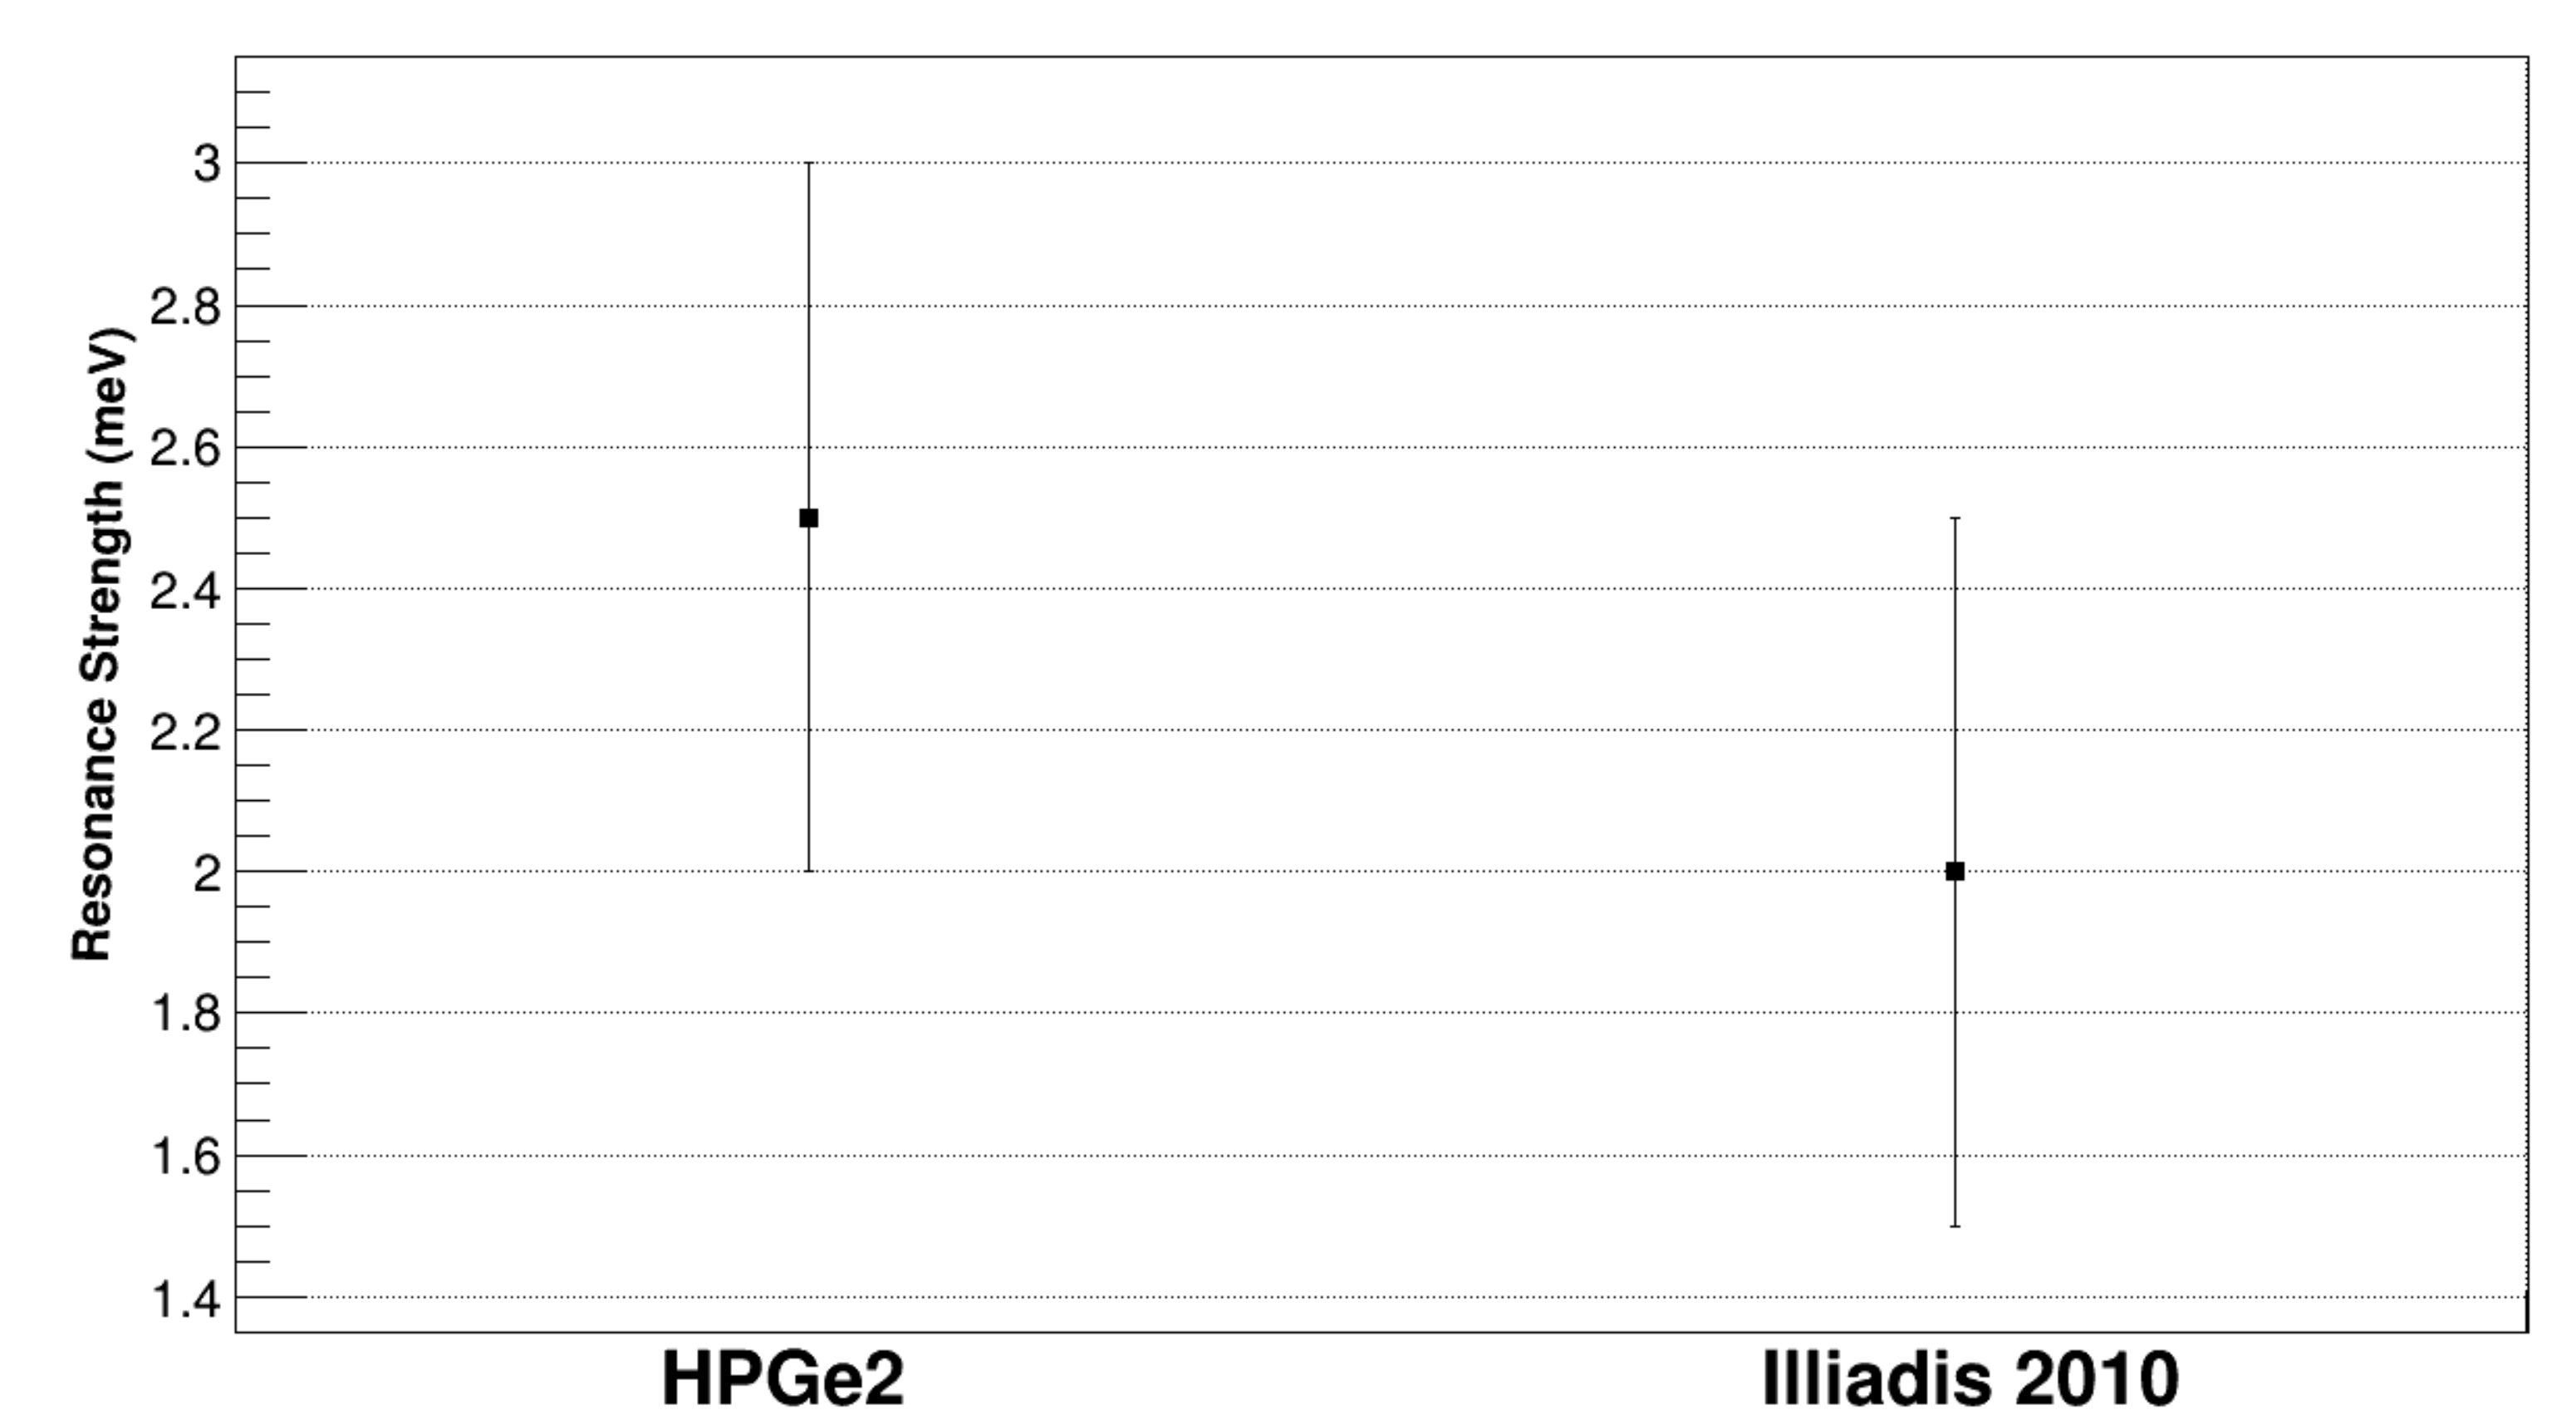
\includegraphics[width=12cm]{res.png}
    \caption{Comparison between $\omega\gamma$ calculated in the report for HPGe2 and value from \cite{Iliadis2010}. }
    \label{fig:res}
\end{figure}



\section{Conclusions}

The 1957 paper by $B^2FH$ revolutionized our understanding of the cosmos, designating stars as the origin of heavy elements. This report, focusing on the \(^{21}\text{Ne}(p,\gamma)^{22}\text{Na}\) reaction, is a result of their findings. Leveraging LUNA's precise replication of stellar conditions, we've analysed and refined the reaction rate measurements and matched resonance strengths with known values. Future accuracy could benefit from factoring in straggling, beam heating, and considering the dual-detector setups. Completing the resonance profile is the next step, vital for a full reaction rate determination, and giving a complete picture of the \reac's role in stellar nucleosynthesis.

\bibliographystyle{unsrt}
\bibliography{refs}




\end{document}